\subsection{Visual and Statistical Analysis of \ce{SiO_2} Distribution in Partitioned Data}\label{sec:visual_analysis}
This section provides a detailed visualization and statistical analysis of the \ce{SiO_2} concentration distribution across data partitions, following the customized k-fold data partitioning procedure described in Section~\ref{subsec:validation_testing_procedures}.
We perform this analysis to validate the consistency of our data partitioning method and to provide a visual understanding of the data distribution it creates.
The analysis focuses on \ce{SiO_2} as a representative example.
We have conducted similar analyses for other oxides, but they are omitted here for brevity.

Figures \ref{fig:histogram_grid_plot} and \ref{fig:histogram_kde_plot} illustrate the histograms and \gls{kde} curves for \ce{SiO_2} concentrations in each training fold, the test set, and their combined distributions.
The consistent histograms and \gls{kde} curves across different training folds indicate that the data distribution within each fold closely matches the overall distribution, confirming their consistency and representativeness.

Figure \ref{fig:original_and_post_fold_plot} contrasts the \ce{SiO_2} concentration distribution before and after data partitioning.
The left plot shows the original distribution, while the right plot displays the fold-assigned distribution, color-coded by fold.
This visualization highlights that the partitioning strategy maintains the overall data distribution while ensuring balanced representation across folds.

\begin{figure*}[h!]
    \centering
    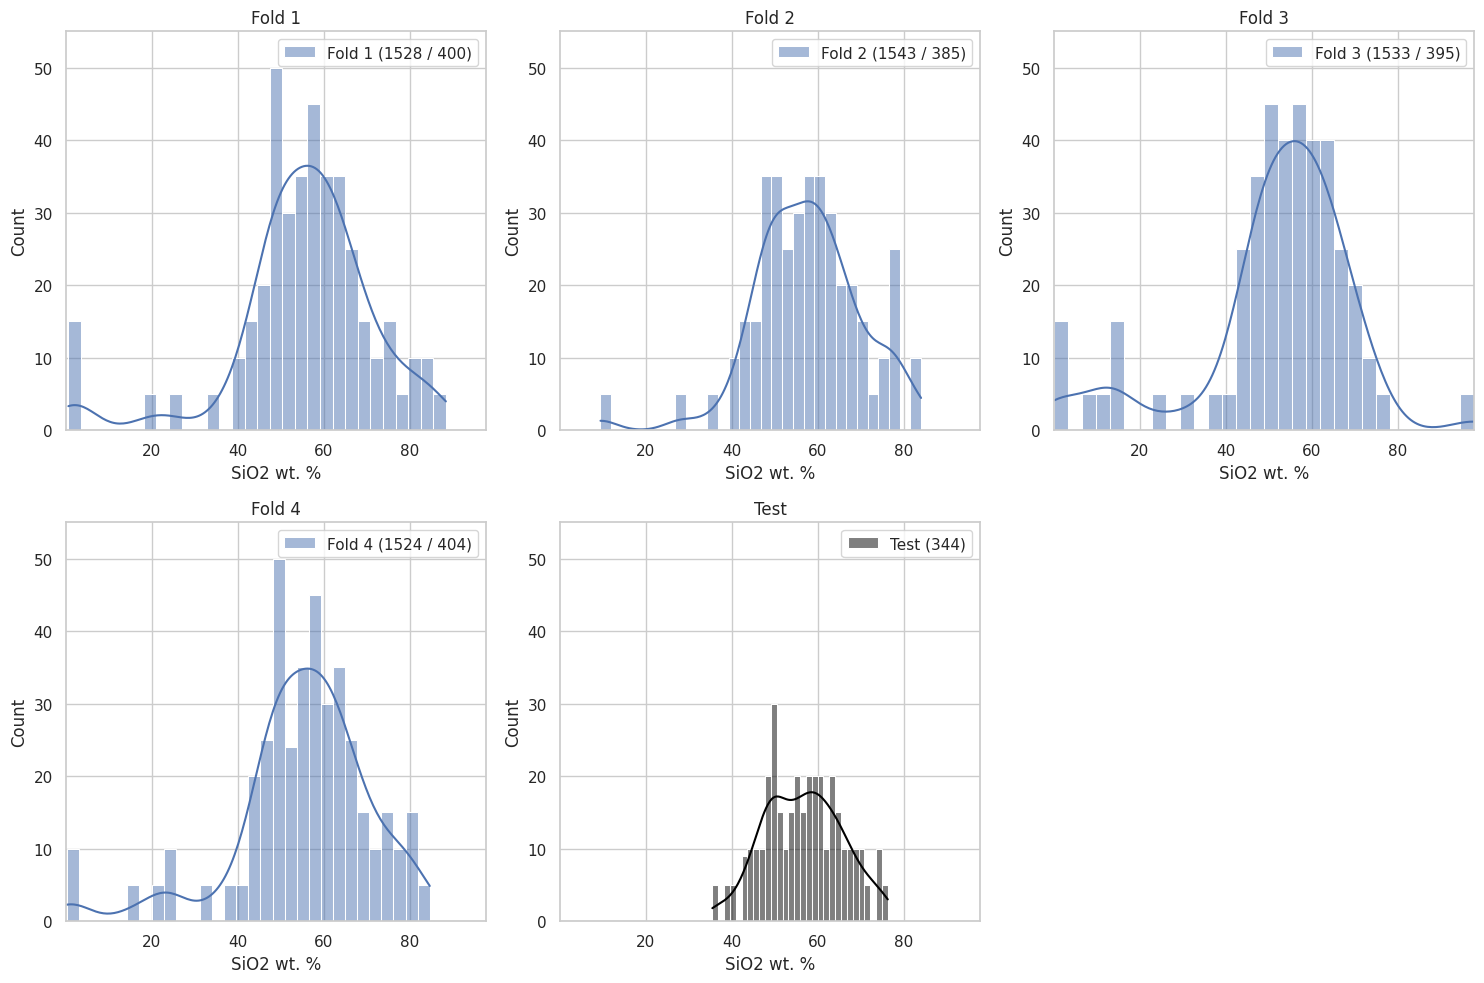
\includegraphics[width=\textwidth]{images/histogram_grid_plot.png}
    \caption{Histogram and \gls{kde} of \ce{SiO_2} Distribution in Each Fold. The y-axis represents the count of samples per bin, and the x-axis represents \ce{SiO_2} concentration. The notation in the legend indicates the amount of instances in the training/validation sets.}
    \label{fig:histogram_grid_plot}
\end{figure*}

\begin{figure*}[h!]
    \centering
    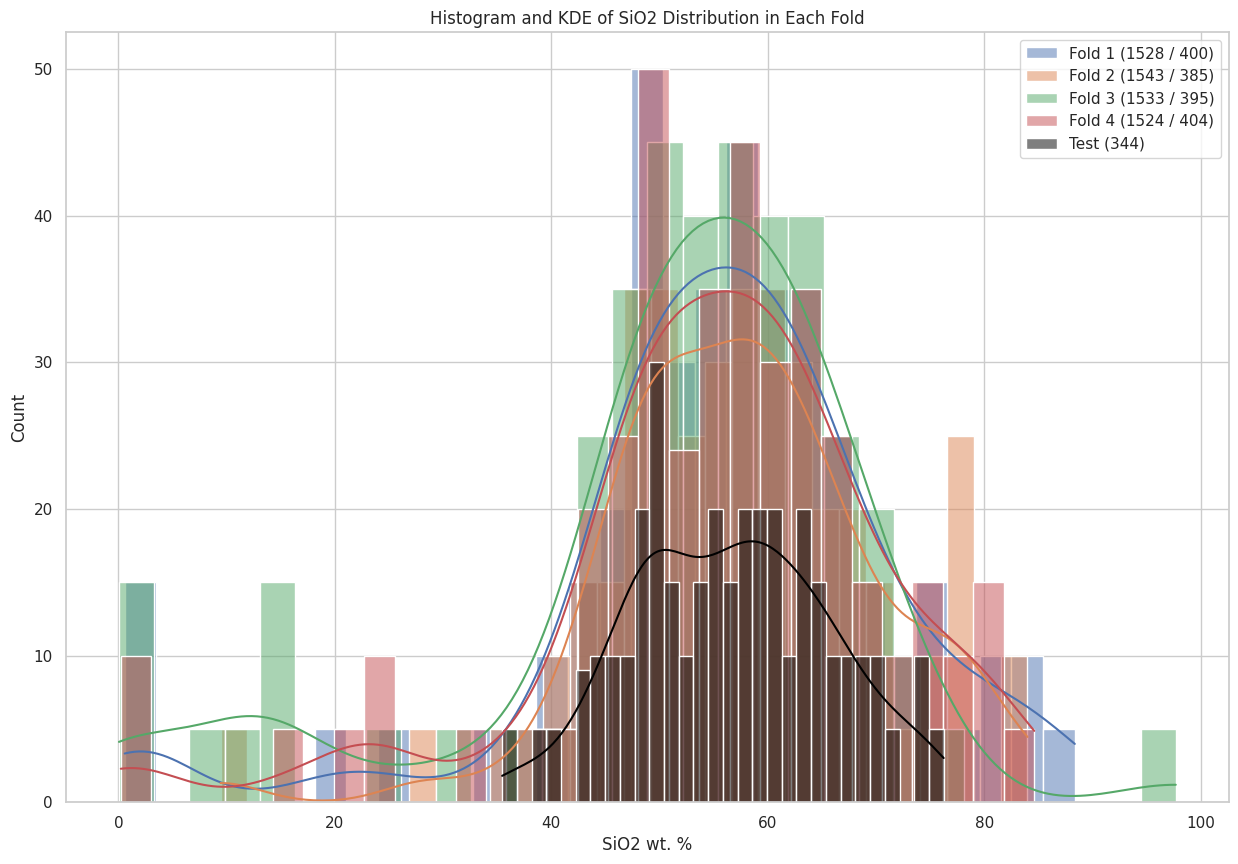
\includegraphics[width=\textwidth]{images/histogram_kde_plot.png}
    \caption{Combined Histogram and \gls{kde} of \ce{SiO_2} Distribution in Each Fold. The y-axis represents the count of samples per bin, and the x-axis represents \ce{SiO_2} concentration. The notation in the legend indicates the amount of instances in the training/validation sets.}
    \label{fig:histogram_kde_plot}
\end{figure*}

\begin{figure*}[h!]
    \centering
    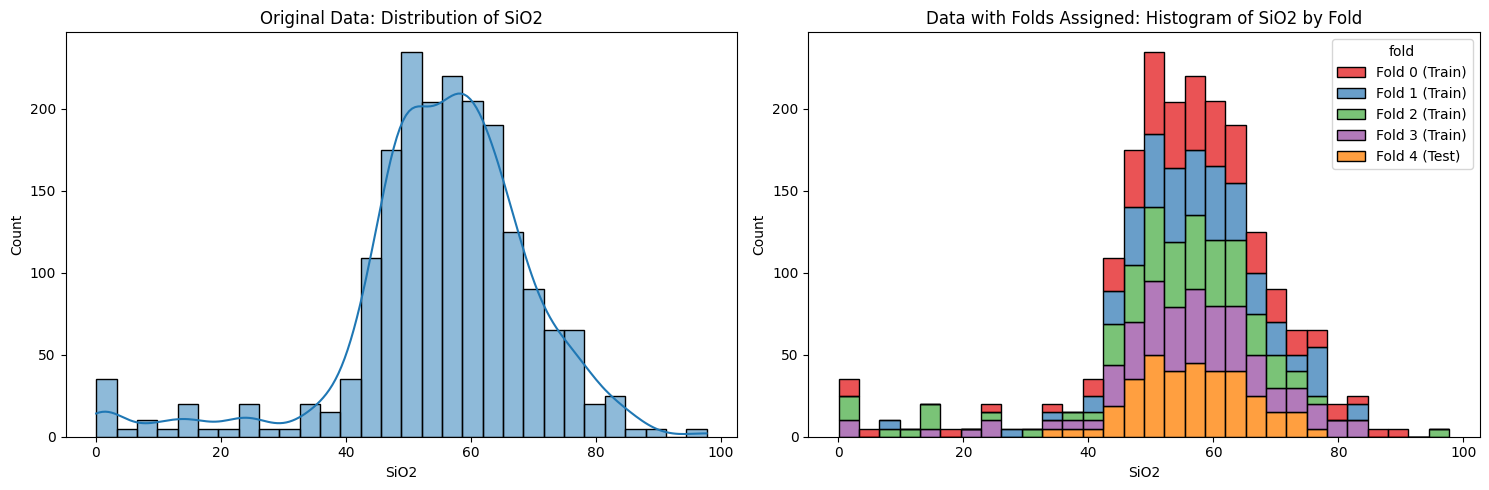
\includegraphics[width=\textwidth]{images/original_and_post_fold.png}
    \caption{Distribution of \ce{SiO_2} concentrations before and after fold assignment. The left plot shows the original distribution of \ce{SiO_2}, while the right plot shows the distribution with folds assigned, color-coded to indicate the different folds.}
    \label{fig:original_and_post_fold_plot}
\end{figure*}


To further validate our visual analysis, we can look at quantitative measures such as the means and standard deviations of \ce{SiO_2} concentrations across the folds and the overall dataset.

\begin{figure*}[htbp]
    \centering
    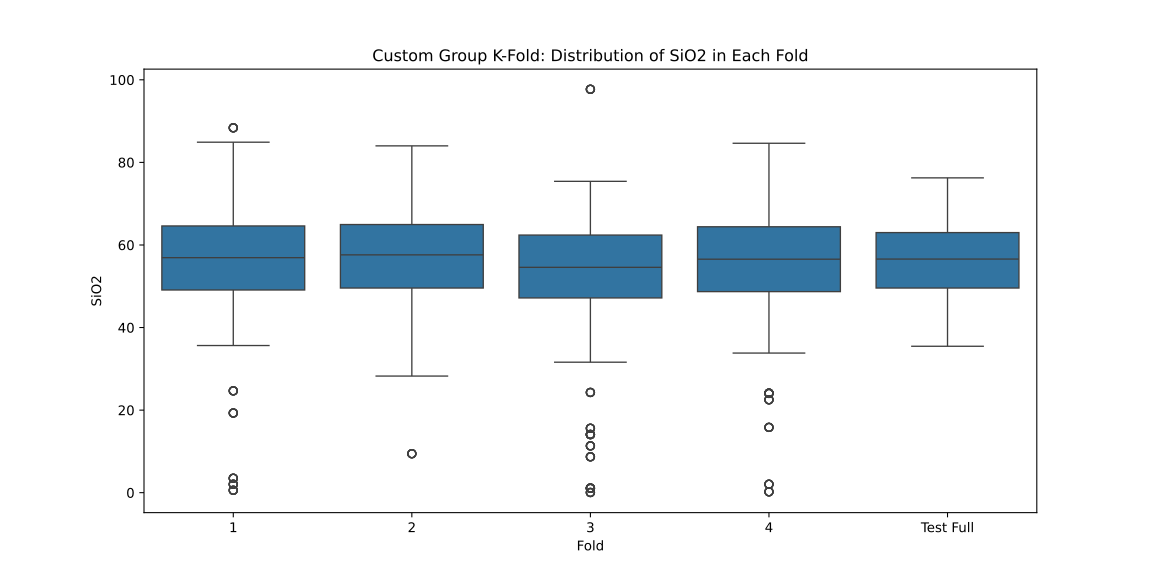
\includegraphics[width=\textwidth]{images/distribution_plot.png}
    \caption{Distribution of \ce{SiO_2} concentrations across cross-validation folds, training set, test set, and the entire dataset. The mean and standard deviation statistics for each partition are indicated figure.}
    \label{fig:siO2_distribution}
\end{figure*}

From Figure~\ref{fig:siO2_distribution}, it is evident that the means and standard deviations of \ce{SiO_2} concentrations for each fold, as well as the combined training set, are consistent with those of the full dataset.
This quantitative consistency supports the visual evidence that each training fold is representative of the entire dataset.
Furthermore, we can see that the standard deviation in the training sets is higher than the standard deviation in the test set, which is expected given the reassignment of extreme values to the training sets.

In conclusion, the visual and statistical analyses presented in this section confirm that our customized k-fold data partitioning procedure effectively maintains balanced and representative distributions across all folds.
This consistency is crucial for the robustness and generalizability of our models, as discussed in Section~\ref{subsec:validation_testing_procedures}.
The alignment between the visual evidence and the quantitative measures reinforces the reliability of our approach, ensuring that our models are well-equipped to perform accurately on unseen data.